\documentclass{beamer}                  %printtaukseen [handout]
\usetheme{Frankfurt}
\usecolortheme{dove}

%\usepackage{pgfpages}                          %printtaukseen
%\pgfpagesuselayout{2 on 1}[a4paper,border shrink=5mm]  %printtaukseen

\usepackage[T1]{fontenc}
\usepackage[utf8]{inputenc}
\usepackage{lmodern}
\usepackage{amssymb}
\usepackage[backend=biber,citestyle=authoryear,bibstyle=authoryear]{biblatex}
\addbibresource{references.bib}
\usepackage{mathtools}
\usepackage{xfrac}
\usepackage[finnish, british]{babel}
\usepackage{cleveref}                       %for multiple refs in one ref
\usepackage{graphicx}
%\usepackage{luximono}
\renewcommand*\familydefault{\ttdefault} %% Only if the base font of the document is to be typewriter style
\usepackage{courier}


%\usepackage[style=authoryear]{biblatex} %for citations
%\bibliographystyle{aer}
%\bibliography{./references/presentationreferences}

\DeclareMathOperator*{\E}{\mathbb{E}}               % Expectation symbol


%%%%% PATHS %%%%%

\graphicspath{{images/}}
%\addbibresource{refs.bib} %for citations

%%%% CUSTOMIZATION OF THE TEMPLATE %%%%%

\useinnertheme{rectangles} %rectangle bullets etc
\beamertemplatenavigationsymbolsempty   %no navigation bar
\setbeamercovered{transparent}      %future bullet points transparent 
\setbeamertemplate{frametitle}[default][colsep=-4bp,rounded=false,shadow=false] %no shadows
\definecolor{dark-gray}{gray}{0.80} %color for the navigation squares

%%%% FOOTLINE CUSTOMIZATION %%%%%

\setbeamercolor{section in head/foot}{fg=black, bg=white}
\makeatletter
\setbeamertemplate{footline}
{
  \leavevmode%
  \hbox{%
  \begin{beamercolorbox}[wd=.333333\paperwidth,ht=2.25ex,dp=1ex,center]{section in head/foot}%
    \usebeamerfont{author in head/foot}\insertshortauthor~~\beamer@ifempty{\insertshortinstitute}{}{(\insertshortinstitute)}
  \end{beamercolorbox}%
  \begin{beamercolorbox}[wd=.333333\paperwidth,ht=2.25ex,dp=1ex,center]{section in head/foot}%
    \usebeamerfont{title in head/foot}\insertshorttitle
  \end{beamercolorbox}%
  \begin{beamercolorbox}[wd=.333333\paperwidth,ht=2.25ex,dp=1ex,right]{section in head/foot}%
    \usebeamerfont{date in head/foot}\insertshortdate{}\hspace*{2em}
    \insertframenumber{} / \inserttotalframenumber\hspace*{2ex} 
  \end{beamercolorbox}}%
  \vskip0pt%
}

%%%% HEADER CUSTOMIZATION %%%%%


\setbeamertemplate{mini frame}
{%
  \begin{pgfpicture}{0pt}{0pt}{.1cm}{.1cm}
    \pgfpathrectangle{\pgfpointorigin}{\pgfpoint{\the\beamer@boxsize}{\the\beamer@boxsize}}
    \pgfusepath{fill,stroke}
  \end{pgfpicture}%
}

\def\slideentry#1#2#3#4#5#6{%
  %section number, subsection number, slide number, first/last frame, page number, part number
  \ifnum#6=\c@part\ifnum#2>0\ifnum#3>0%
    \ifbeamer@compress%
      \advance\beamer@xpos by1\relax%
    \else%
      \beamer@xpos=#3\relax%
      \beamer@ypos=#2\relax%
    \fi%
  \hbox to 2pt{%
    \beamer@tempdim=-\beamer@vboxoffset%
    \advance\beamer@tempdim by-\beamer@boxsize%
    \multiply\beamer@tempdim by\beamer@ypos%
    \advance\beamer@tempdim by -.05cm%
    \raise\beamer@tempdim\hbox{%
      \beamer@tempdim=\beamer@boxsize%
      \multiply\beamer@tempdim by\beamer@xpos%
      \advance\beamer@tempdim by -\beamer@boxsize%
      \advance\beamer@tempdim by 1pt%
      \kern\beamer@tempdim
      \global\beamer@section@min@dim\beamer@tempdim
      \hbox{\beamer@link(#4){%
          \usebeamerfont{mini frame}%
          \ifnum\c@section>#1%
            \color{dark-gray}%
          \else%
            \ifnum\c@section=#1%
              \ifnum\c@subsection>#2%
                \color{dark-gray}%
              \else%
                \ifnum\c@subsection=#2%
                  \ifnum\c@subsectionslide>#3%
                    \color{dark-gray}%
                  \else%
                    \color{fg}%
                  \fi%
                \else%
                  \color{dark-gray}%
                \fi%
              \fi%
            \else%
              \color{dark-gray}%
            \fi%
          \fi%
          \usebeamertemplate{mini frame}%
        }}}\hskip-10cm plus 1fil%
  }\fi\fi%
  \else%
  \fakeslideentry{#1}{#2}{#3}{#4}{#5}{#6}%
  \fi\ignorespaces
  }
  
%%%% SOME BUG %%%%%

\def\pdftex@driver{pdftex.def}
\ifx\Gin@driver\pdftex@driver
  \def\pgfsys@color@unstacked#1{%
    \pdfliteral{\csname\string\color@#1\endcsname}%
  }
\fi

\makeatother



%%%%% INFORMATION ABOUT THE DOCUMENT %%%%%

\title[Final - FTI]{Fundamentos Teóricos de Informática}
\author[PATM]{Pablo Toledo}
\institute[UNPSJB]{UNPSJB}         
\date{Feb 27, 2014}

                      
%%%%% ACTUAL DOCUMENT PAGES %%%%%                     

\begin{document}

    \frame{\titlepage}
    \begin{frame}
        \frametitle{Máquinas de Turing}

        \center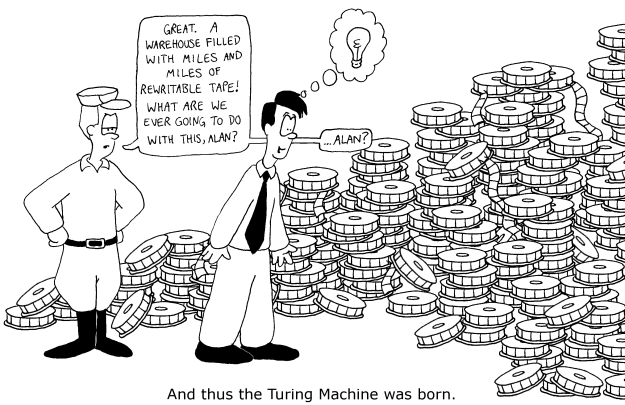
\includegraphics[height=189px]{turing}
        \endcenter
    \end{frame}
    \begin{frame}
        \frametitle{¿Qué es una TM?}
        \begin{itemize}
            \item Un modelo que define una \textit{Máquina abstracta} que manipula símbolos sobre una (o más cintas) de acuerdo a un conjunto de reglas.
        \end{itemize}
        \center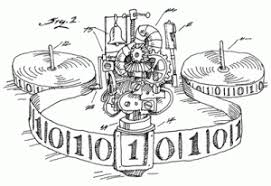
\includegraphics[height=120px]{turingmachine}
    \end{frame}
    \begin{frame}
        \frametitle{Máquinas de Turing (cont...)}
        \begin{itemize}
            \item Inventada en 1936 por Alan Turing
            \item Con esta se puede probar las limitaciones fundamentales de los algoritmos
            \item En particular, Turing la utilizó para resolver el \textbf{Halting Problem} o \textbf{Problema de la Detención}... y ganar WW2 (y probablemente haber salvado al mundo)
        \end{itemize}
    \end{frame}

    \begin{frame}
    \center
\includegraphics[width=200px]{zac}
    \endcenter 
    \end{frame}

    \begin{frame}
        \frametitle{¿Pero cómo es una Máquina de Turing?}
        Una Máquina de Turing es una quintupla
        \center
        $T=(S,\sum,\delta,s_{0},F)$
        \endcenter
        Donde
        \begin{itemize}
            \item $S$ es el conjunto de estados posibles
            \item $\sum$ es el alfabeto de trabajo
            \item $\delta$ es una funcion parcial $\delta:S \times \sum \rightarrow S \times \sum \times \{ I, N, D\}$
                
                Donde
                \begin{itemize}
                    \item I denota movimiento a la izquierda
                    \item D denota movimiento a la derecha
                    \item N sin movimiento
                \end{itemize}
            \item $F \subseteq S$ es el conjunto de estados finalizadores

        \end{itemize}
    \end{frame}
    
    \begin{frame}
        \frametitle{Configuración}
        Llamaremos configuración de una $T=(S,\sum,\delta,s_{0},F)$ a una terna $(s,\alpha,i)$ donde $s$ es el estado acutal de $T$, $\alpha \in \sum^{*}$ (la secuencia de caracteres acutalmente sobre la cinta) e $i \in \mathbb{Z}^{+}$ siendo la posición de la cabeza lectora en la cinta.
    \end{frame}

    \begin{frame}
        \frametitle{Transición}
        Una transición de una Máquina T será representada por la relación $\vdash$ entre configuraciones: 
        $(s,\alpha,i) \vdash (s',\alpha',i')$ si existe en T una regla de transición $\delta(s,\alpha) = (s',\alpha,M)$ donde $s,s' \in S; \alpha, \alpha' \in \sum^{*}; M \in \{I, N, D\}$ e
        \begin{equation}
            i' = 
            \begin{cases}
                i-1 & \text{si M=I} \\
                i & \text{si M=N}\\
                i+1 & \text{si M=D}\\
            \end{cases}
        \end{equation}
    \end{frame}
    \begin{frame}
        \frametitle{Aceptación de una cadena y Lenguaje}
        \textbf{Definición}\\

        Se dice que $w$ es reconocida por $T=(S,\sum,\delta,s_{0},F)$ si $(s_{0},w,1) \vdash^{*} (s_{f},\alpha,i)$ para algún $s_{f} \in F, w, \alpha \in \sum^{*}, i \in \mathbb{Z}^{+}$

        \bigskip

        \textbf{Definición}

        Dado un alfabeto $\sum$ y un lenguaje $L \subseteq \sum^{*}$, $L$ es aceptado por $T=(S,\sum,\delta,s_{0},F)$ si:

    $L = L(T) = \{w|w \in \sum^{*} \text{y w es aceptada por} T\}$

    En tal caso diremos que $L$ es un lenguaje \textbf{Turing Aceptable}

    \end{frame}
    \begin{frame}
        \frametitle{MT para computar funciones}
        \textbf{Definición}\\

        Se dice que una funcion $f_{T} : \sum^{*} \rightarrow \sum^{*}$ es Turing-Computable por una MT si existe una MT $T=(S,\sum,\delta,s_{0},F)$ tal que:

        $(s_{0},x,1) \vdash^{*} (s_{f},f_{T}(x),i)$ donde $w \in \sum, i \in \mathbb{Z}$ y $s_{f} \in F$
    \end{frame}
    \begin{frame}
        \frametitle{Computabilidad}

        Sea $\sum$ un alfabeto y sean $Y,N$ dos símbolos fuera de éste ($\notin \sum$). Un lenguaje $L \subseteq \sum^{*}$ se dice \textit{decibile por una Máquina de Turing} o \textit{Turing-Decidible} si y sólo si la función $X_{L}: \sum \rightarrow \{Y, N\}$ es Turing-computable, y para cada $w \in \sum^{*}$, da una respuesta acorde

        \begin{equation}
            X_{L}(w)=_{def}
            \begin{cases}
                \text{Y si w $\in$ L}\\

                \text{N si w $\notin$ L}\\
            \end{cases}
        \end{equation}
        
    \end{frame}
    \begin{frame}
        \frametitle{Máquina de Turing NO Determinista}
        
        Una máquina de Turing no determinista se puede definir de la siguiente manera:

        \bigskip

        $T=(S,\sum,\delta,s_{0},F)$ 

        \bigskip

        Donde todos los elementos son los mismos de una Máquina de Turing determinista, salvo que $\delta$ se define de la siguiente manera

        \bigskip

        $\delta : S\times \sum \rightarrow P(S\times\sum\times\{I, D ,N\})$

    \end{frame}
    \begin{frame}

    \textbf{Teorema}
    Para cada máquina de Turing no determinista T nd podemos construir una máquina de Turing determinista T d equivalente.

    \end{frame}
    \begin{frame}

    \textbf{Tesis 1} (de Turing)\\
    
    Un proceso naturalmente llamadopro cedimiento efectivo puede ser realizado por una máquina de Turing, es decir es Turing Computable.

    \bigskip

    \textbf{Tesis 2} (de Church)\\
    Los procesos naturalmente llamados procedimientos efectivos o las funciones efectivamente computables son identificados con la clase de Funciones Recursivas Parciales.

    \end{frame}
    \begin{frame}
        \begin{itemize}
            \item Teoría de Funciones Recursivas Parciales de K. Godel y S. Kleene (1936)
            \item Cálculo Lambda de Alonzo Church (1941).
            \item Sistemas Canónicos de Post(1943).
            \item Redes de Petri (1962)
        \end{itemize}

    \end{frame}
    \begin{frame}
    \center
\includegraphics[width=200px]{eq}
    \endcenter 
    \end{frame}
    \begin{frame}
    \center
\includegraphics[width=200px]{hack0}
    \endcenter 
    \end{frame}
    \begin{frame}

\textbf{Definición}\\
Denominaremos Problema de Decisión a aquellos formulados a traves de una pregunta y que requieren una respuesta de tipo Si/No.
    \bigskip

\textbf{Definición}\\
Un problema de decisión se dice Soluble si existe un algoritmo total para determinar si la propiedad es verdadera.
    \bigskip

    \end{frame}
    \begin{frame}
    \center
\includegraphics[width=200px]{halt}
    \endcenter 
    \end{frame}
    \begin{frame}

\textbf{Definición}\\
Un problema de decisión se dice Parcialmente Soluble si existe un procedimiento efectivo para determinar si la propiedad es verdadera.
    \bigskip

\textbf{Definición}\\
Un problema de decisión es Insoluble si no existe un procedimiento efectivo para determinar si la propiedad es válida.
    \bigskip

    \end{frame}
    \begin{frame}

\textbf{Definición}\\
Sean una máquina de Turing T y una cadena $\alpha$, el problema de la detención de las máquinas de Turing se define como: ¿Existe un algoritmo para decidir si T se detendrá comenzando en el estado inicial con $\alpha$ en la cinta?

    \bigskip
\textbf{Teorema}\\
El Problema de la Detención es Algorítmicamente Insoluble
    \bigskip
    \end{frame}
    \begin{frame}

\textbf{Definición}\\
Sean dos problemas de decisión, $PD_{1}$ y $PD_{2}$ , diremos que el problema de decisión $PD_{1}$ se reduce al problema de decisión $PD_{2}$ y lo escribiremos $PD_{1}\rightarrow_{reduct}$ $PD_{2}$ si un algoritmo para
solucionar $PD_{2}$ puede ser usado para construir la solución de
$PD_{1}$ .
    \bigskip

\textbf{Teorema}\\

Sean $PD_{1}$ y $PD_{2}$ dos problemas de decisión, se cumple lo siguiente:
1. Si $PD_{1} \rightarrow_{reduct}$ $PD_{2}$ y $PD_{2}$ es soluble, entonces $PD_{1}$
también lo es.
2. Si $PD_{1} \rightarrow PD_{2}$ es insoluble, entonces $PD_{2}$ también lo es.

    \end{frame}


\printbibliography
%\addcontentsline{toc}{section}{References}
\clearpage
\end{document}
              
            
